\documentclass[../main.tex]{subfiles}
\begin{document}
% \section{Presentation and Overview}
\section{概述}

\begin{tkzexample}[latex=5cm,small]
\begin{tikzpicture}[scale=.25]
  \tkzDefPoints{00/0/A,12/0/B,6/12*sind(60)/C}
  \foreach \density in {20,30,...,240}{%
  \tkzDrawPolygon[fill=teal!\density](A,B,C)
  \pgfnodealias{X}{A}
  \tkzDefPointWith[linear,K=.15](A,B) \tkzGetPoint{A}
  \tkzDefPointWith[linear,K=.15](B,C) \tkzGetPoint{B}
  \tkzDefPointWith[linear,K=.15](C,X) \tkzGetPoint{C}}
\end{tikzpicture}
\end{tkzexample}

\vspace*{12pt}

% \subsection{Why \tkzname{\tkznameofpack}?}
\subsection{为什么要开发\tkzname{\tkznameofpack}?}

% My initial goal was to provide other mathematics teachers and myself with a tool
% to quickly create Euclidean geometry figures without investing too much effort
% in learning a new programming language.
% Of course, \tkzname{\tkznameofpack}  is for math teachers who use \LATEX\ and
% makes it possible to easily create correct  drawings by means of \LATEX.

开发该宏包的最初想法是为自己和其它数学老师设计一个\LATEX{}绘图工具,以实现欧氏几何图形的
快速绘制,而不需要费力学习和掌握一门新的绘图语言。
当然,\tkzname{\tkznameofpack}适用于所有使用\LATEX{}的教师,以实现在\LATEX{}中
轻松、正确地欧氏几何绘图。


% It appeared that the simplest method was to reproduce the one used to obtain
% construction by hand.
显然,最简单的绘图方法是按手工绘图的方式和思维进行绘图。
% To describe a construction, you must, of course, define the objects but also the
% actions that you perform. It seemed to me that syntax close to the language of
% mathematicians and their students would be more easily understandable; moreover,
% it also seemed to me that this syntax should be close to that of \LaTeX.
% The objects, of course, are points, segments, lines, triangles, polygons and
% circles. As for actions, I considered five to be sufficient, namely: define,
% create, draw, mark and label.
为描述一个几何图形,须定义图形对象以及对这些对象所执行的操作。因此,如果与数学家或学习数学的
学生使用的数学语言语法相近,这些语法则更容易理解和掌握。当然,宏包的语法也必须
符合\LATEX{}用户的使用习惯。

基于此,该宏包定义了点、线段、直线、三角形、多边形和圆六种图形对象。并且设计了
定义、创建、绘制、标记和标注五个对图形对象的基本操作。

% The syntax is perhaps too verbose but it is, I believe, easily accessible.
% As a result, the students like teachers were able to easily access this tool.
虽然这会使语法比较冗长,但却更容易理解和使用。因此,
用户能够轻松使用该宏包提供的命令进行绘图。
% \subsection{\tkzname{\tkznameofpack}  vs \tkzname{\TIKZ}}
\subsection{\tkzname{\tkznameofpack}与\tkzname{\TIKZ}}

% I love programming with  \TIKZ,  and without  \TIKZ\  I would never have had the
% idea to create \tkzname{\tkznameofpack}  but never forget that behind it there
% is  \TIKZ\  and that it is always possible to insert code from  \TIKZ.
% \tkzname{\tkznameofpack}  doesn't prevent you from using  \TIKZ.
当然,\TIKZ{}本身的绘图功能也极其强大,如果没有\TIKZ{}的话,则永远不会有\tkzname{\tkznameofpack}
宏包。\tkzname{\tkznameofpack}是基于\TIKZ{}开发的,并且可以在\tkzname{\tkznameofpack}绘图代
码中随时使用\TIKZ{}代码,\tkzname{\tkznameofpack}并不限制对\TIKZ{}的直接调用。
% That said, I don't think mixing syntax is a good thing.
不过,并不建议采用混合语法绘图,这样会降低代码的可读性。

% There is no need to compare \TIKZ\  and \tkzname{\tkznameofpack}.  The latter is
% not addressed to the same audience as  \TIKZ. The first one allows you to do a
% lot of things, the second one only does geometry drawings. The first one can do
% everything the second one does, but the second one will more easily do what you
% want.
其实,无需比较\TIKZ{}和\tkzname{\tkznameofpack},两者的用户不完全相同。前者可以实现
更为复杂的图形绘制,后者则擅长绘制欧氏几何图形。当然,前者完全能够实现后者所有的功能。

% \subsection{How it works}
\subsection{工作模式}

%\subsubsection{Example Part I: gold triangle}
\subsubsection{示例I: 黄金三角形}


\begin{center}
\begin{tikzpicture}
% 坐标点定义
\tkzDefPoint(0,0){C} % 也可以使用\tkzDefPoint[label=below:$C$](0,0){C}通过参数直接标注,但不建议这样做
\tkzDefPoint(2,6){B}
% 通过坐标旋转定义D点和E点
\tkzDefPointBy[rotation= center B angle 36](C) \tkzGetPoint{D}
\tkzDefPointBy[rotation= center B angle 72](C) \tkzGetPoint{E}
% 通过求直线交点定义A点
\tkzInterLL(B,E)(C,D) \tkzGetPoint{A}
\tkzInterLL(C,E)(B,D) \tkzGetPoint{H}
% 绘制
\tkzDrawArc[delta=10](B,C)(E)
\tkzDrawPolygon(C,B,D)
\tkzDrawSegments(D,A B,A C,E)
% 标记
\tkzMarkAngles(C,B,D E,A,D) % 绘制圆弧
\tkzLabelAngles[pos=1.5](C,B,D E,A,D){$\alpha$}
\tkzMarkRightAngle(B,H,C)
\tkzDrawPoints(A,...,E)
% 仅做标注
\tkzLabelPoints[below left](C,A)
\tkzLabelPoints[below right](D)
\tkzLabelPoints[above](B,E)
\end{tikzpicture}
\end{center}

% Let's analyze the figure
其绘制过程如下:
% \begin{enumerate}
% \item $CBD$ and $DBE$ are isosceles triangles;
%
% \item $BC=BE$ and $(BD)$ is a bisector of the angle $CBE$;
%
% \item From this we deduce that the $CBD$ and $DBE$ angles are equal and have
% the same measure $\alpha$
%    \[\widehat{BAC} +\widehat{ABC} + \widehat{BCA}=180^\circ \ \text{in the
% triangle}\ BAC \]
%    \[3\alpha + \widehat{BCA}=180^\circ\  \text{in the triangle}\ CBD\]
%    then
%      \[\alpha + 2\widehat{BCA}=180^\circ \]
%    or
%      \[\widehat{BCA}=90^\circ -\alpha/2 \]
%
% \item Finally \[\widehat{CBD}=\alpha=36^\circ \]
%      the triangle $CBD$ is a \enquote{gold} triangle.
% \end{enumerate}
\begin{enumerate}
  \item $CBD$和$DBE$都是等腰三角形;
  \item $BC=BE$,$BD$是角$CBE$的角平分线。
  \item 由此推出角$CBD$和角$DBE$相等,在此,记为 $\alpha$。
	  \[\widehat{BAC} +\widehat{ABC} + \widehat{BCA}=180^\circ \text{(在三
	  角形}BAC\text{中)}\]
	  \[3\alpha + \widehat{BCA}=180^\circ  \text{(在三角形} CBD\text{中)}\]
   因此
   \[\alpha + 2\widehat{BCA}=180^\circ \]
   或
   \[\widehat{BCA}=90^\circ -\alpha/2 \]
 \item 从而可得   \[\widehat{CBD}=\alpha=36^\circ \]
	 所以,$CBD$是一个\enquote{黄金}三角形。
\end{enumerate}

\vspace*{24pt}
% How construct a gold triangle or an angle of $36^\circ$?
如何构造一个黄金三角形或者顶角为$36^\circ$的等腰三角形呢?

\begin{enumerate}
% \item We place the fixed points $C$ and $D$. |\tkzDefPoint(0,0){C}| and
% |\tkzDefPoint(4,0){D}|;
\item 先使用|\tkzDefPoint(0,0){C}|和|\tkzDefPoint(4,0){D}|定义两个已知点 $C$ 和 $D$。
% \item  We construct a square $CDef$ and we construct the midpoint $m$ of $[Cf]$;
\item 构造一个正方形$CDef$,并且取$Cf$的中点$m$。当然,可以使用圆规和直尺来完成所有这些工作。
% We can do all of this with a compass and a rule;
% \item Then we trace an arc with center $m$ through $e$. This arc cross the
% line $(Cf)$ at $n$;
\item 然后,以$m$为圆心作过$e$的圆弧,该圆弧与直线$Cf$相交于$n$
% \item Now the two arcs with center $C$ and $D$ and radius $Cn$ define the
% point $B$.
\item 至此,分别以 $C$和$D$为圆心,以$Cn$为半径的两个圆弧可定义点$B$。
\end{enumerate}

\begin{minipage}{0.4\textwidth}
\begin{tikzpicture}
\tkzDefPoint(0,0){C}
\tkzDefPoint(4,0){D}
\tkzDefSquare(C,D)
\tkzGetPoints{e}{f}
\tkzDefMidPoint(C,f)
\tkzGetPoint{m}
\tkzInterLC(C,f)(m,e)
\tkzGetSecondPoint{n}
\tkzInterCC[with nodes](C,C,n)(D,C,n)
\tkzGetFirstPoint{B}
\tkzDrawSegment[brown,dashed](f,n)
\pgfinterruptboundingbox
\tkzDrawPolygon[brown,dashed](C,D,e,f)
\tkzDrawArc[brown,dashed](m,e)(n)
\tkzCompass[brown,dashed,delta=20](C,B)
\tkzCompass[brown,dashed,delta=20](D,B)
\endpgfinterruptboundingbox
\tkzDrawPoints(C,D,B)
\tkzDrawPolygon(B,...,D)
\end{tikzpicture}
\end{minipage}
\begin{minipage}{0.58\textwidth}
\begin{tkzexample}[code only,small]
\begin{tikzpicture}
  \tkzDefPoint(0,0){C}
  \tkzDefPoint(4,0){D}
  \tkzDefSquare(C,D)
  \tkzGetPoints{e}{f}
  \tkzDefMidPoint(C,f)
  \tkzGetPoint{m}
  \tkzInterLC(C,f)(m,e)
  \tkzGetSecondPoint{n}
  \tkzInterCC[with nodes](C,C,n)(D,C,n)
  \tkzGetFirstPoint{B}
  \tkzDrawSegment[brown,dashed](f,n)
  \pgfinterruptboundingbox
  \tkzDrawPolygon[brown,dashed](C,D,e,f)
  \tkzDrawArc[brown,dashed](m,e)(n)
  \tkzCompass[brown,dashed,delta=20](C,B)
  \tkzCompass[brown,dashed,delta=20](D,B)
  \endpgfinterruptboundingbox
  \tkzDrawPoints(C,D,B)
  \tkzDrawPolygon(B,...,D)
\end{tikzpicture}
\end{tkzexample}
\end{minipage}

% After building the golden triangle $BCD$, we build the point $A$ by noticing
% that $BD=DA$. Then we get the point $E$ and finally the point $F$. This is done
% with already intersections of defined objects  (line and circle).
构造了黄金三角形$BCD$后,可以通过以$D$为圆心,$BD$为半径的圆与直线$CD$的
交点来定义$BD=DA$的点$A$。 再通过以$B$为圆心,$BC$为半径的圆与直线$BA$的
交点来定义的然后再定义点$E$。最后通过直线$BA$与直线$BD$的交点定义点$ F $。

\begin{center}
\begin{tikzpicture}
\tkzDefPoint(0,0){C}
\tkzDefPoint(4,0){D}
\tkzDefSquare(C,D)
\tkzGetPoints{e}{f}
\tkzDefMidPoint(C,f)
\tkzGetPoint{m}
\tkzInterLC(C,f)(m,e)
\tkzGetSecondPoint{n}
\tkzInterCC[with nodes](C,C,n)(D,C,n)
\tkzGetFirstPoint{B}
\tkzInterLC(C,D)(D,B) \tkzGetSecondPoint{A}
\tkzInterLC(B,A)(B,D) \tkzGetSecondPoint{E}
\tkzInterLL(B,D)(C,E) \tkzGetPoint{F}
\tkzDrawPoints(C,D,B)
\tkzDrawPolygon(B,...,D)
\tkzDrawPolygon(B,C,D)
\tkzDrawSegments(D,A A,B C,E)
\tkzDrawArc[delta=10](B,C)(E)
\tkzMarkRightAngle[fill=blue!20](B,F,C)
\tkzFillAngles[fill=blue!10](C,B,D E,A,D)
\tkzMarkAngles(C,B,D E,A,D)
\tkzLabelAngles[pos=1.5](C,B,D E,A,D){$\alpha$}
\tkzLabelPoints[below](A,C,D,E)
\tkzLabelPoints[above right](B,F)
\tkzDrawPoints(A,...,F)
\end{tikzpicture}
\end{center}

\begin{tkzexample}[code only,small,pre={},post={}]
\begin{tikzpicture}
  \tkzDefPoint(0,0){C}
  \tkzDefPoint(4,0){D}
  \tkzDefSquare(C,D)
  \tkzGetPoints{e}{f}
  \tkzDefMidPoint(C,f)
  \tkzGetPoint{m}
  \tkzInterLC(C,f)(m,e)
  \tkzGetSecondPoint{n}
  \tkzInterCC[with nodes](C,C,n)(D,C,n)
  \tkzGetFirstPoint{B}
  \tkzInterLC(C,D)(D,B) \tkzGetSecondPoint{A}
  \tkzInterLC(B,A)(B,D) \tkzGetSecondPoint{E}
  \tkzInterLL(B,D)(C,E) \tkzGetPoint{F}
  \tkzDrawPoints(C,D,B)
  \tkzDrawPolygon(B,...,D)
  \tkzDrawPolygon(B,C,D)
  \tkzDrawSegments(D,A A,B C,E)
  \tkzDrawArc[delta=10](B,C)(E)
  \tkzDrawPoints(A,...,F)
  \tkzMarkRightAngle[fill=blue!20](B,F,C)
  \tkzFillAngles[fill=blue!10](C,B,D E,A,D)
  \tkzMarkAngles(C,B,D E,A,D)
  \tkzLabelAngles[pos=1.5](C,B,D E,A,D){$\alpha$}
  \tkzLabelPoints[below](A,C,D,E)
  \tkzLabelPoints[above right](B,F)
\end{tikzpicture}
\end{tkzexample}

% \subsubsection{Example Part II: two others methods gold and euclide triangle}
\subsubsection{示例II: 另外两种黄金三角形绘制方式}

% \tkzname{\tkznameofpack} knows how to define a \enquote{gold} or \enquote{euclide} triangle. We
% can define $BCD$ and $BCA$ like gold triangles.
\tkzname{\tkznameofpack}宏包可以通过\enquote{gold}或\enquote{euclide}选项定义三角形,因此可按如下方式定义$BCD$和$BCA$黄金三角形:

\begin{tkzexample}[code only,small,pre={},post={}]
\begin{tikzpicture}
  \tkzDefPoint(0,0){C}
  \tkzDefPoint(4,0){D}
  \tkzDefTriangle[euclide](C,D)
  \tkzGetPoint{B}
  \tkzDefTriangle[euclide](B,C)
  \tkzGetPoint{A}
  \tkzInterLC(B,A)(B,D) \tkzGetSecondPoint{E}
  \tkzInterLL(B,D)(C,E) \tkzGetPoint{F}
  \tkzDrawPoints(C,D,B)
  \tkzDrawPolygon(B,...,D)
  \tkzDrawPolygon(B,C,D)
  \tkzDrawSegments(D,A A,B C,E)
  \tkzDrawArc[delta=10](B,C)(E)
  \tkzDrawPoints(A,...,F)
  \tkzMarkRightAngle[fill=blue!20](B,F,C)
  \tkzFillAngles[fill=blue!10](C,B,D E,A,D)
  \tkzMarkAngles(C,B,D E,A,D)
  \tkzLabelAngles[pos=1.5](C,B,D E,A,D){$\alpha$}
  \tkzLabelPoints[below](A,C,D,E)
  \tkzLabelPoints[above right](B,F)
\end{tikzpicture}
\end{tkzexample}

% Here is a final method that uses rotations:
也可以使用坐标旋转的方法定义三角形:

\begin{tkzexample}[code only,small,pre={},post={}]
\begin{tikzpicture}
  \tkzDefPoint(0,0){C} % 也可以在定义点的同时用
  % 类似\tkzDefPoint[label=below:$C$](0,0){C}的方式进行标注
  % 但不建议这样做
  \tkzDefPoint(2,6){B}
  % 通过旋转定义点D和点E
  \tkzDefPointBy[rotation= center B angle 36](C) \tkzGetPoint{D}
  \tkzDefPointBy[rotation= center B angle 72](C) \tkzGetPoint{E}
  % 通过直线交点定义点A和点H
  \tkzInterLL(B,E)(C,D) \tkzGetPoint{A}
  \tkzInterLL(C,E)(B,D) \tkzGetPoint{H}
  % 绘制
  \tkzDrawArc[delta=10](B,C)(E)
  \tkzDrawPolygon(C,B,D)
  \tkzDrawSegments(D,A B,A C,E)
  % 角度标记
  \tkzMarkAngles(C,B,D E,A,D) % 绘制圆弧
  \tkzLabelAngles[pos=1.5](C,B,D E,A,D){$\alpha$}
  \tkzMarkRightAngle(B,H,C)
  \tkzDrawPoints(A,...,E)
  % 仅实现标注
  \tkzLabelPoints[below left](C,A)
  \tkzLabelPoints[below right](D)
  \tkzLabelPoints[above](B,E)
\end{tikzpicture}
\end{tkzexample}

% \subsubsection{Complete but minimal example}
\subsubsection{最小工作示例}

% A unit of length being chosen, the example shows how to obtain a segment of
% length $\sqrt{a}$ from a segment of length $a$, using a ruler and a compass.
该示例说明了如何使用尺规绘图的方式从长度为$a$的线段得到长度为$\sqrt{a}$的线段

$IB=a$, $AI=1$

\vspace{12pt}
\hypertarget{firstex}{}

\begin{tikzpicture}[scale=1,ra/.style={fill=gray!20}]
  % 已知点
  \tkzDefPoint(0,0){A}
  \tkzDefPoint(1,0){I}
  % 求解点
  \tkzDefPointBy[homothety=center A ratio  10 ](I) \tkzGetPoint{B}
  \tkzDefMidPoint(A,B)              \tkzGetPoint{M}
  \tkzDefPointWith[orthogonal](I,M) \tkzGetPoint{H}
  \tkzInterLC(I,H)(M,B)             \tkzGetSecondPoint{C}
  % 绘图
  \tkzDrawSegment[style=orange](I,C)
  \tkzDrawArc(M,B)(A)
  \tkzDrawSegment[dim={$1$,-16pt,}](A,I)
  \tkzDrawSegment[dim={$a/2$,-10pt,}](I,M)
  \tkzDrawSegment[dim={$a/2$,-16pt,}](M,B)
  % 标记
  \tkzMarkRightAngle[ra](A,I,C)
  % 标注
  \tkzDrawPoints(I,A,B,C,M)
  \tkzLabelPoint[left](A){$A(0,0)$}
  \tkzLabelPoints[above right](I,M)
  \tkzLabelPoints[above left](C)
  \tkzLabelPoint[right](B){$B(10,0)$}
  \tkzLabelSegment[right=4pt](I,C){$\sqrt{a^2}=a \ (a>0)$}
\end{tikzpicture}

% \emph{Comments}
\emph{建议}

\begin{itemize}
% \item The Preamble
\item 导言区

% Let us first look at the preamble. If you need it, you have to load
% \tkzname{xcolor} before \tkzname{tkz-euclide}, that is, before \TIKZ. \TIKZ\ may
% cause problems with the active characters, but\dots
% provides a library in its latest version that's supposed to solve these
% problems \NameLib{babel}.
如果需要使用\tkzname{xcolor}宏包,则必须在\tkzname{tkz-euclide}之前载入该宏包,也就是
在\TIKZ{}宏包之前载入。否则可能会与\TIKZ{}宏包冲突,但\TIKZ{}宏包提供的\NameLib{babel}
库能解决这些冲突。

\begin{tkzltxexample}[small]
\documentclass{standalone} % 或其它文档类
% \usepackage{xcolor} % 需要在tikz或tkz-euclide宏包之前载入
\usepackage{tkz-euclide} % 不再需要显式载入TikZ宏包
% \usetkzobj{all}  不再需要该命令
% \usetikzlibrary{babel} 如果有冲突,则可以使用该库进行解决
\end{tkzltxexample}

% The following code consists of several parts:
该代码可以分解为以下几个部分:

% \item Definition of fixed points: the first part includes the definitions of
% the points necessary for the construction, these are the fixed points. The
% macros \tkzcname{tkzInit} and \tkzcname{tkzClip} in most cases are not
% necessary.
\item 定义已知点:第1部分是定义已知点:
多数情况下,并不需要使用\tkzcname{tkzInit}和\tkzcname{tkzClip}命令。

\begin{tkzltxexample}[]
  \tkzDefPoint(0,0){A}
  \tkzDefPoint(1,0){I}
\end{tkzltxexample}

% \item The second part is dedicated to the creation of new points from the
% fixed points;
% a $B$ point is placed at $10$~cm from $A$. The middle of $[AB]$ is defined
% by $M$ and then the orthogonal line to the $(AB)$ line is searched for at the
% $I$ point. Then we look for the intersection of this line with the semi-circle
% of center $M$ passing through $A$.
\item 第2部分是利用已知点通过计算得到其它点:
$B$点位于从$A$开始的$10$~cm处。 $M$是线段$[AB]$的中点,然后得到通过$I$点的直线$(AB)$的正交直线。
从而得到该正交线与以$M$为圆心,过$A$点的半圆的交点。

\begin{tkzltxexample}[small]
  \tkzDefPointBy[homothety=center A ratio 10](I)
    \tkzGetPoint{B}
  \tkzDefMidPoint(A,B)
    \tkzGetPoint{M}
  \tkzDefPointWith[orthogonal](I,M)
    \tkzGetPoint{H}
  \tkzInterLC(I,H)(M,B)
    \tkzGetSecondPoint{C}
\end{tkzltxexample}

% \item The third one includes the different drawings;
\item 第3部分是图形绘制:
\begin{tkzltxexample}[small]
  \tkzDrawSegment[style=orange](I,C)
  \tkzDrawArc(M,B)(A)
  \tkzDrawSegment[dim={$1$,-16pt,}](O,I)
  \tkzDrawSegment[dim={$a/2$,-10pt,}](A,M)
  \tkzDrawSegment[dim={$a/2$,-16pt,}](M,B)
  \tkzDrawPoints(I,A,B,C,M)
\end{tkzltxexample}

% \item  Marking: the fourth is devoted to marking;
\item 第4部分是绘制标记:

\begin{tkzltxexample}[small]
  \tkzMarkRightAngle(A,I,C)
\end{tkzltxexample}

% \item Labelling: the latter only deals with the placement of labels.
\item 最后是布置标注:
\begin{tkzltxexample}[small]
  \tkzLabelPoint[left](A){$A(0,0)$}
  \tkzLabelPoints[above right](I,M)
  \tkzLabelPoints[above left](C)
  \tkzLabelPoint[right](B){$B(10,0)$}
  \tkzLabelSegment[right=4pt](I,C){$\sqrt{a^2}=a \ (a>0)$}
\end{tkzltxexample}

% \item The full code:
\item 完整的代码:

\begin{tkzexample}[code only,small,pre={},post={},small]
\begin{tikzpicture}[scale=1,ra/.style={fill=gray!20}]
  % 已知点
  \tkzDefPoint(0,0){A}
  \tkzDefPoint(1,0){I}
  % 求解点
  \tkzDefPointBy[homothety=center A ratio  10 ](I) \tkzGetPoint{B}
  \tkzDefMidPoint(A,B)              \tkzGetPoint{M}
  \tkzDefPointWith[orthogonal](I,M) \tkzGetPoint{H}
  \tkzInterLC(I,H)(M,B)             \tkzGetSecondPoint{C}
  % 绘图
  \tkzDrawSegment[style=orange](I,C)
  \tkzDrawArc(M,B)(A)
  \tkzDrawSegment[dim={$1$,-16pt,}](A,I)
  \tkzDrawSegment[dim={$a/2$,-10pt,}](A,M)
  \tkzDrawSegment[dim={$a/2$,-16pt,}](M,B)
  \tkzDrawPoints(I,A,B,C,M)
  % 标记
  \tkzMarkRightAngle[ra](A,I,C)
  % 标注
  \tkzLabelPoint[left](A){$A(0,0)$}
  \tkzLabelPoints[above right](I,M)
  \tkzLabelPoints[above left](C)
  \tkzLabelPoint[right](B){$B(10,0)$}
  \tkzLabelSegment[right=4pt](I,C){$\sqrt{a^2}=a \ (a>0)$}
\end{tikzpicture}
\end{tkzexample}
\end{itemize}

\newpage

% \subsection{The Elements of tkz code}
\subsection{tkz的基本要素}

% In this paragraph, we start looking at the \enquote{rules} and \enquote{symbols} used to create
% a figure with \tkzname{\tkznameofpack}.
% 接下来,讨论使用\tkzname{\tkznameofpack}绘制图形时的\enquote{规则}和\enquote{符号系统}

% The primitive objects are points. You can refer to a point at any time using
% the name given when defining it. (it is possible to assign a different name
% later on).
\tkzname{\tkznameofpack}绘图中的基本要素是点,可以在任何时候通过定义一个点时命名该点,并通过该点的名称引用一个点
(当然,也可以在后续操作中为点赋于不同的名称)。

\medskip
% In general, \tkzname{\tkznameofpack} macros have a name beginning with tkz.
% There are four main categories starting with:
% |\tkzDef|\dots|\tkzDraw|\dots|\tkzMark|\dots{} and |\tkzLabel|\dots
通常,\tkzname{\tkznameofpack}的命令都是以tkz为前缀,其主要四类前缀是:
|\tkzDef|\dots{}、|\tkzDraw|\dots{}、|\tkzMark|\dots{}和|\tkzLabel|\dots{}

% Among the first category, |\tkzDefPoint| allows you to define fixed points. It
% will be studied in detail later. Here we will see in detail the macro
% |\tkzDefTriangle|.
在第1类命令中,|\tkzDefPoint|命令用于通过坐标定义一个点,该命令的细节过后会进行详细讨论。
在此,首先详细讨论|\tkzDefTriangle|命令。

% This macro makes it possible to associate to a pair of points a third point in
% order to define a certain triangle |\tkzDefTriangle(A,B)|. The obtained point is
% referenced |tkzPointResult| and it is possible to choose another reference with
% |\tkzGetPoint{C}| for example.
% Parentheses are used to pass arguments. In |(A,B)| $A$ and $B$ are the points
% with which a third will be defined.
该命令利用一个点与一对已知点的关系,通过已知类型的三角形来定义这个点。
可以通过|tkzPointResult|使用该点,当然,也可以通过|\tkzGetPoint{C}|保存并为该点命名,以便后续引用该点。
命令中的圆括号用于传递参数,例如在|(A,B)|中的$A$和$B$是已知点,用于根据三角形类型定义第三个点。

% However, in |{C}| we use braces to retrieve the new point.
% In order to choose a certain type of triangle among the following choices:
% |equilateral|, |half|, |pythagoras|, |school|, |golden| or |sublime|, |euclide|,
% |gold|, |cheops|\dots{} and |two angles| you just have to choose between hooks,
% for example can be used: |\tkzDefTriangle[euclide](A,B)| |\tkzGetPoint{C}|
然而,在|\tkzGetPoint{C}|命令中,用大括号中的参数命名新点,三角形类型有:
|equilateral|、|half|、 |pythagoras|、 |school|、 |golden| 或 |sublime|、 |euclide|、
|gold|、 |cheops|\dots{} 和 |two angles|,
例如: |\tkzDefTriangle[euclide](A,B)| |\tkzGetPoint{C}|

\begin{minipage}{0.48\textwidth}
\begin{tikzpicture}[scale=0.75]
  \tkzDefPoints{0/0/A,8/0/B}
  \foreach \tr in {equilateral,half,pythagore,%
          school,golden,euclide, gold,cheops}
  {\tkzDefTriangle[\tr](A,B) \tkzGetPoint{C}
  \tkzDrawPoint(C)
  \tkzLabelPoint[right](C){\tr}
  \tkzDrawSegments(A,C C,B)}
  \tkzDrawPoints(A,B)
  \tkzDrawSegments(A,B)
\end{tikzpicture}
\end{minipage}
\begin{minipage}{0.51\textwidth}
\begin{tkzexample}[code only,small]
\begin{tikzpicture}[scale=0.75]
  \tkzDefPoints{0/0/A,8/0/B}
  \foreach \tr in {equilateral,half,pythagore,%
           school,golden,euclide, gold,cheops}
    {\tkzDefTriangle[\tr](A,B) \tkzGetPoint{C}
  \tkzDrawPoint(C)
  \tkzLabelPoint[right](C){\tr}
  \tkzDrawSegments(A,C C,B)}
  \tkzDrawPoints(A,B)
  \tkzDrawSegments(A,B)
\end{tikzpicture}
\end{tkzexample}
\end{minipage}

% \subsection{Notations and conventions}
\subsection{符号和约定}

% I deliberately chose to use the geometric French and personal  conventions  to
% describe the geometric objects represented. The objects defined and represented
% by \tkzname{\tkznameofpack} are points, lines and circles located in a plane.
% They are the primary objects of Euclidean geometry from which we will construct
% figures.
该宏包选用法国的几何符号和作者习惯描述几何图形,
\tkzname{\tkznameofpack}宏包定义和表示的对象有平面中的点、线和圆,
它们是欧氏几何的主要元素,可以根据这些基本元素构成欧氏几何图形。

% According to \tkzimp{Euclidian} these figures will only illustrate pure ideas
% produced by our brain.
根据欧几里得的定义,仅使用这些基本图形就可以构成各种复杂图形。
% Thus a point has no dimension and therefore no real existence. In the same way
% the line has no width and therefore no existence in the real world. The objects
% that we are going to consider are only representations of ideal mathematical
% objects. \tkzname{\tkznameofpack} will follow the steps of the ancient Greeks to
% obtain geometrical constructions using the ruler and the compass.
因此,一个点并没有具体的尺寸,它在现实中不存在。同样,一条线也没有宽度,也不存在。
在\tkzname{\tkznameofpack}宏包中需要考虑的是代表理想数学概念的对象,
\tkzname{\tkznameofpack}遵循古希腊尺规作图的方式进行绘图。

% Here are the notations that will be used:
以下是使用的基本符号:

\begin{itemize}
% \item The points are represented geometrically either by a small disc or by the
% intersection of two lines (two straight lines, a straight line and a circle or
% two circles). In this case, the point is represented by a cross.
\item 点可以用圆盘或十字线(两条直线、一条直线和圆或两个圆的交点)表示。

\newpage

\begin{tkzexample}[latex=6cm, small]
\begin{tikzpicture}
  \tkzDefPoints{0/0/A,4/2/B}
  \tkzDrawPoints(A,B)
  \tkzLabelPoints(A,B)
\end{tikzpicture}
\end{tkzexample}

% or else
或

\begin{tkzexample}[latex=6cm, small]
\begin{tikzpicture}
  \tkzSetUpPoint[shape=cross, color=red]
  \tkzDefPoints{0/0/A,4/2/B}
  \tkzDrawPoints(A,B)
  \tkzLabelPoints(A,B)
\end{tikzpicture}
\end{tkzexample}

% The existence of a point being established, we can give it a label which will be
% a capital letter (with some exceptions) of the Latin alphabet such as $A$, $B$
% or $C$. For example:
对于一个点,可以使用类似$A$、$B$或$C$这样的大写字母(当然,也会有例外)进行标注,例如:

% \begin{itemize}
% \item $O$ is a center for a circle, a rotation, etc.;
% \item $M$ defined a midpoint;
% \item $H$ defined the foot of an altitude;
% \item $P'$ is the image of $P$ by a transformation ;
% \end{itemize}
\begin{itemize}
\item $O$ 可以表示圆心、旋转中心等;
\item $M$ 可以表示中点;
\item $H$ 可以表示高;
\item $P'$ 可以表示变换后,点$P$的镜像点;
\end{itemize}

% It is important to note that the reference name of a point in the code may be
% different from the label to designate it in the text. So we can define a point A
% and give it as label $P$. In particular the style will be different, point A
% will be labeled $A$.
需要注意的是:一个点在代码中的引用名称和标注名称可能不一样,
所以可以定义一个点A,但是将其标注为$P$。

\begin{tkzexample}[latex=6cm, small]
\begin{tikzpicture}
  \tkzDefPoints{0/0/A}
  \tkzDrawPoints(A)
  \tkzLabelPoint(A){$P$}
\end{tikzpicture}
\end{tkzexample}

% Exceptions: some points such as the middle of the sides of a triangle share a
% characteristic, so it is normal that their names also share a common character.
% We will designate these points by $M_a$, $M_b$ and $M_c$ or $M_A$, $M_B$ and
% $M_C$.
注意也有例外情况:一些如三角形各边的中点,应带有边的特征,因此,常常用带有边特征的标注,如:
$M_a$、 $M_b$ 和$M_c$ 或 $M_A$、 $M_B$ 和$M_C$。

% In the code, these points will be referred to as: M\_A, M\_B and M\_C.
在代码中,可以使用诸如M\_A、M\_B和M\_C的形式命名并引用这些点。

% Another exception relates to intermediate construction points which will not be
% labelled. They will often be designated by a lowercase letter in the code.
另外一种例外情况是无需标注的内部点,这些点在代码中常常用小写字母表示。

% \item The line segments are designated by two points representing their ends in
% square brackets: $[AB]$.
\item 线段使用方括号中的两个点表示,如:$[AB]$。

% \item The straight lines are in Euclidean geometry defined by two points so $A$
% and $B$ define the straight line $(AB)$. We can also designate this stright line
% using the Greek alphabet and name it $(\delta)$ or $(\Delta)$. It is also
% possible to designate the straight line with lowercase letters such as $d$ and
% $d'$.
\item 在欧氏几何中,直线用两个点表示,因此,点$A$和点$B$定义的直线表示为$(AB)$。
也可以使用希腊字母表示直线,并将其命名为$(\delta)$ 或 $(\Delta)$。
也可以使用小写字母表示直线,如$d$和$d'$。

% \item The semi-straight line is designated as follows $[AB)$.
\item 射线可表示为$[AB)$.

% \item Relation between the straight lines. Two perpendicular $(AB)$ and $(CD)$
% lines will be written $(AB) \perp (CD)$ and if they are parallel we will write
% $(AB) \parallelslant (CD)$.
\item 对于直线间的关系,例如对于直线$(AB)$和直线$(CD)$,垂直表示为$(AB) \perp (CD)$,
平行表示为$(AB) \parallelslant (CD)$。

% \item The lengths of the sides of triangle ABC are $AB$, $AC$ and $BC$. The
% numbers are also designated by a lowercase letter so we will write: $AB=c$,
% $AC=b$ and $BC=a$. The letter $a$ is also used to represent an angle, and $r$ is
% frequently used to represent a radius, $d$ a diameter, $l$ a length, $d$ a
% distance.
\item 三角形ABC的边长表示为$AB$、$AC$和$BC$。长度值一般用小写字母表示
如:$AB=c$、$AC=b$和$BC=a$。字母$a$也常常用于表示一个角度,$r$常常用于表示半径,
$d$表示直径,$l$表示长度,$d$也可以表示距离。

% \item Polygons are designated afterwards by their vertices so $ABC$ is a
% triangle, $EFGH$ a quadrilateral.
\item 多边形用其顶点表示,如三角形表示为$ABC$,四边形表示为$EFGH$。

% \item Angles are generally measured in degrees (ex $60^\circ$) and in an
% equilateral $ABC$ triangle we will write $\widehat{ABC}=\widehat{B}=60^\circ$.
\item 角度的单位是度(例如:$60^\circ$),对于等边三角形$ABC$,
可以表示为$\widehat{ABC}=\widehat{B}=60^\circ$。

% \item The arcs are designated by their extremities. For example if $A$ and $B$
% are two points of the same circle then $\widearc{AB}$.
\item 圆弧用起止点表示,如,若$A$和$B$是同一个圆上的两个点,则可以用$\widearc{AB}$表示圆弧。

% \item Circles are noted either $\mathcal{C}$ if there is no possible confusion
% or $\mathcal{C}$ $(O~;~A)$ for a circle with center $O$ and passing through the
% point $A$ or $\mathcal{C}$ $(O~;~1)$ for a circle with center O and radius 1 cm.
\item 如果没有岐义,一个圆可以表示为$\mathcal{C}$,
或用$\mathcal{C}$ $(O~;~A)$表示圆心在$O$点并通过点$A$的圆
或用$\mathcal{C}$ $(O~;~1)$表示圆心在点O半径为1 cm的圆。

% \item  Name of the particular lines of a triangle: I used the terms bisector,
% bisector out, mediator (sometimes called perpendicular bisectors), altitude,
% median and symmedian.
\item  三角形中的特殊线有:内角角平分线、外角角平分线等。

% \item ($x_1$,$y_1$) coordinates of the point $A_1$, ($x_A$,$y_A$) coordinates of
% the point $A$.
\item ($x_1$,$y_1$)表示点$A_1$的坐标分量,($x_A$,$y_A$)表示点$A$的坐标分量。

\end{itemize}


% \subsection{How to use the \tkzname{\tkznameofpack} package?}
\subsection{使用\tkzname{\tkznameofpack}宏包}

% \subsubsection{Let's look at a classic example}
\subsubsection{经典示例}

% In order to show the right way, we will see how to build an equilateral
% triangle. Several possibilities are open to us, we are going to follow the steps
% of Euclid.
在此,以绘制一个等边三角形为例,展示\tkzname{\tkznameofpack}宏包的正确使用方式。
当然,绘制该图形可以有多种方式,本例中将遵循欧氏几何尺规绘图步骤。

\begin{itemize}
% \item First of all you have to use a document class. The best choice to test
% your code is to create a single figure with the class \tkzname{standalone}\index{standalone}.
\item 首先需要引入文档类,对于单个图形而言,
比较方便的一种方式是使用\tkzname{standalone}\index{standalone}文档类。

\begin{verbatim}
\documentclass{standalone}
\end{verbatim}

% \item Then load the \tkzname{\tkznameofpack} package:
\item 然后载入\tkzname{\tkznameofpack}宏包:

\begin{verbatim}
\usepackage{tkz-euclide}
\end{verbatim}

% You don't need to load \TIKZ\ because the \tkzname{\tkznameofpack} package
% works on top of TikZ and loads it.
注意,由于\tkzname{\tkznameofpack}宏包是基于\TIKZ{}宏包开发的,
会同时载入该宏包,因此,无需再次载入\TIKZ{}宏包
\item {\color{red} \bomb \sout{|\BS usetkzobj\{all\}|}},
% With the new version 3.03 you don't need this line anymore. All objects are now
% loaded.
在3.03版以后,无需再使用该命令载入绘图对象,默认情况下会载入所有对象。
% \item Start the document and open a TikZ picture environment:
\item 开始文档,并使用tikzpicture环境绘制欧氏几何图形:

\begin{verbatim}
\begin{document}
\begin{tikzpicture}
\end{verbatim}

% \item Now we define two fixed points:
\item 定义两个已知点:

\begin{verbatim}
\tkzDefPoint(O,O){A}
\tkzDefPoint(5,2){B}
\end{verbatim}

% \item Two points define two circles, let's use these circles:
% \item Two points define two circles, let's use these circles:
%
% circle with center $A$ through $B$ and circle with center $B$ through $A$.
% These two circles have two points in common.
\item 使用这两个点定义两个圆,并使用这两个圆定义交点:

$(A,B)$表示以$A$点为圆心通过$B$点,$(B,A)$表示以$B$点为圆心通过$A$点,
两个圆共用这$A$点和$B$点。

\begin{verbatim}
\tkzInterCC(A,B)(B,A)
\end{verbatim}

% We can get the points of intersection with
得到两个圆的交点,并命名为$C$和$D$

\begin{verbatim}
\tkzGetPoints{C}{D}
\end{verbatim}

% \item All the necessary points are obtained, we can move on to the final steps
% including the plots.
\item 至此,便完成了所有点的定义,接下来进行绘图。

\begin{verbatim}
\tkzDrawCircles[gray,dashed](A,B B,A)
\tkzDrawPolygon(A,B,C)% 三角形
\end{verbatim}

% \item Draw all points $A$, $B$, $C$ and $D$:
\item 绘制$A$、 $B$、 $C$和$D$:

\begin{verbatim}
\tkzDrawPoints(A,...,D)
\end{verbatim}

% \item The final step, we print labels to the points and use options for
% positioning:\par
\item 绘制标注,在绘制标注时,可以为其指定位置参数。

\begin{verbatim}
\tkzLabelSegments[swap](A,B){$c$}
\tkzLabelPoints(A,B,D)
\tkzLabelPoints[above](C)
\end{verbatim}

% \item We finally close both environments
\item 最后,结束各个环境

\begin{verbatim}
\end{tikzpicture}
\end{document}
\end{verbatim}

% \item The complete code
\item 完整的代码

\begin{tkzexample}[latex=8cm,small]
\begin{tikzpicture}[scale=0.5]
  % 已知点
  \tkzDefPoint(0,0){A}
  \tkzDefPoint(5,2){B}
  % 计算得到的点
  \tkzInterCC(A,B)(B,A)
  \tkzGetPoints{C}{D}
  % 绘图
  \tkzDrawCircles[gray,dashed](A,B B,A)
  \tkzDrawPolygon(A,B,C)
  \tkzDrawPoints(A,...,D)
  % 标记
  \tkzMarkSegments[mark=s||](A,B B,C C,A)
  % 标注
  \tkzLabelSegments[swap](A,B){$c$}
  \tkzLabelPoints(A,B,D)
  \tkzLabelPoints[above](C)
\end{tikzpicture}
\end{tkzexample}

\end{itemize}

% \subsubsection{\tkzname{Set, Calculate, Draw, Mark, Label}}
\subsubsection{点集、计算、绘制、标记和标注}

% The title could have been: \texttt{Separation of Calculus and Drawings}
该标题的含义是:\texttt{计算与绘制分离}

% When a document is prepared using the \LATEX\ system, the source code of the
% document can be divided into two parts: the document body and the preamble.
% Under this methodology,  publications can be structured, styled and typeset with
% minimal effort.
在使用\LATEX{}排版时,源代码分为导言和正文两大部分。
通过这种方式,可以将排版内容进行结构化设计,并通过样式和排版命令集简化用户的排版过程。
% I propose a similar methodology for creating figures with \tkzname{\tkznameofpack}.
\tkzname{\tkznameofpack}正是基于这种内容与格式分离思想进行设计的,以简化用户绘图过程。

% The first part defines the fixed points, the second part allows the creation of
% new points. These are the two main parts. All that is left to do is to draw,
% mark and label.
首先定义已知点,然后计算其他点,这是绘图的两个主要内容。
接下来是绘制、标记和标注。

\end{document}
\endinput
